\newpage
\section{Khảo sát các giải pháp đã có}
\subsection{Khảo sát các ứng dụng, sản phẫm hoặc hệ thống liên quan}
\subsubsection*{PHÂN TÍCH NHÓM GIẢI PHÁP TRỌN GÓI TỪ CÁC TẬP ĐOÀN CÔNG NGHỆ QUỐC TẾ (INTERNATIONAL TURNKEY SOLUTIONS)}
Nhóm giải pháp này đại diện cho đỉnh cao của công nghệ nông nghiệp (AgriTech) thế giới, được phát triển bởi các tập đoàn đa quốc gia với bề dày kinh nghiệm hàng thập kỷ. Đặc điểm chung là tính đồng bộ tuyệt đối (Ecosystem), độ tin cậy cao và khả năng xử lý dữ liệu nông học phức tạp, nhưng đi kèm với chi phí đầu tư và vận hành lớn.

\subsubsection*{Netafim NetBeat™ (Israel)  Hệ điều hành canh tác kỹ thuật số khép kín}
\begin{figure}[H]
    \centering
    \includegraphics[width=0.9\textwidth]{img/quocte1.png}
    \caption{Nông trại Netafim NetBeat™}
\end{figure}
\textbf{Mục tiêu và triết lý thiết kế}
\begin{itemize}
\item NetBeat™ được định vị như "bộ não" của nông trại, tích hợp Giám sát – Phân tích – Điều khiển trong một vòng lặp khép kín.
\item Hướng tới các trang trại quy mô lớn và nhà kính công nghệ cao, yêu cầu độ chính xác tuyệt đối về dinh dưỡng.
\end{itemize}

\textbf{Kiến trúc hệ thống và tính năng kỹ thuật}
\begin{itemize}
\item Phần cứng điều khiển trung tâm (NetMCU): thiết bị đạt chuẩn công nghiệp, có khả năng Edge Computing, đảm bảo vận hành ngay cả khi mất Internet.
\item Mô hình cây trồng động (Dynamic Crop Models™): sử dụng cơ sở dữ liệu nông học hơn 50 năm để tự động điều chỉnh nước và phân bón theo giai đoạn sinh trưởng và thời tiết.
\item Hệ sinh thái mở: cho phép tích hợp cảm biến bên thứ ba (NDVI, hình ảnh vệ tinh, diệp lục tố).
\end{itemize}

\textbf{Trải nghiệm người dùng và giao diện}
\begin{itemize}
\item Dashboard trực quan với bản đồ số và mã màu trạng thái khu tưới.
\item Trợ lý ảo đưa ra khuyến nghị hành động cụ thể.
\item Quản lý và điều khiển hoàn toàn từ xa qua smartphone hoặc tablet.
\end{itemize}

\textbf{Đánh giá phù hợp}
\begin{itemize}
\item \textbf{Ưu điểm:} hệ thống đồng bộ, độ bền và độ tin cậy rất cao.
\item \textbf{Nhược điểm:} chi phí đầu tư và phí SaaS lớn.
\item \textbf{Khuyến nghị:} phù hợp cho nhà đầu tư vốn lớn, định hướng xuất khẩu chất lượng cao.
\end{itemize}

\subsubsection*{Fujitsu Akisai (Nhật Bản)  Mô hình đám mây nông nghiệp chính xác}
\begin{figure}[H]
    \centering
    \includegraphics[width=0.9\textwidth]{img/quocte2.png}
    \caption{Nông trại Fujitsu Akisai}
\end{figure}
\textbf{Mục tiêu và triết lý thiết kế}
\begin{itemize}
\item Tiếp cận nông nghiệp như sản xuất công nghiệp, mọi yếu tố được kiểm soát bằng dữ liệu.
\item Đã triển khai thực tế tại Việt Nam thông qua hợp tác với FPT.
\end{itemize}

\textbf{Kiến trúc và tính năng}
\begin{itemize}
\item Quản lý môi trường canh tác bằng mạng cảm biến dày đặc (nhiệt độ, độ ẩm, CO\textsubscript{2}, ánh sáng, dinh dưỡng).
\item Hỗ trợ canh tác từ xa với chuyên gia Nhật Bản thông qua dữ liệu và video.
\item Tích hợp chuỗi cung ứng, truy xuất nguồn gốc toàn diện.
\end{itemize}

\textbf{Đánh giá phù hợp}
\begin{itemize}
\item \textbf{Ưu điểm:} SOP chuẩn hóa cao, chất lượng sản phẩm đồng đều.
\item \textbf{Nhược điểm:} chi phí vận hành rất cao, khó tùy biến cho cây trồng nhiệt đới.
\item \textbf{Khuyến nghị:} phù hợp cho doanh nghiệp lớn, sản xuất nông sản chức năng hoặc xuất khẩu sang Nhật.
\end{itemize}

\subsubsection*{PHÂN TÍCH NHÓM GIẢI PHÁP NỀN TẢNG CÔNG NGHỆ TRONG NƯỚC (DOMESTIC INTEGRATED PLATFORMS)}
Nhóm giải pháp được “may đo” cho điều kiện Việt Nam, cân bằng giữa công nghệ, chi phí và tập quán canh tác.

\subsubsection*{Rynan Technologies  Hệ sinh thái nông nghiệp số Mê Kông}
\textbf{Định hướng}
\begin{itemize}
\item Tập trung giải quyết bài toán xâm nhập mặn, nuôi tôm công nghệ cao và lúa giảm phát thải.
\item Thiết bị IoT bền bỉ, phù hợp môi trường nước mặn và khí hậu khắc nghiệt.
\end{itemize}

\textbf{Tính năng nổi bật}
\begin{itemize}
\item Giám sát côn trùng thông minh bằng AI và Computer Vision.
\item Quan trắc phát thải Methane phục vụ tín chỉ carbon.
\item Quan trắc môi trường nước liên tục qua 4G.
\end{itemize}

\textbf{Đánh giá}
\begin{itemize}
\item \textbf{Ưu điểm:} sát thực tế Việt Nam, giá thành hợp lý.
\item \textbf{Khuyến nghị:} rất phù hợp cho nuôi trồng thủy sản và lúa tại ĐBSCL.
\end{itemize}

\subsubsection*{MimosaTEK – Tiên phong tưới chính xác cho cây trồng cạn}
% \begin{figure}[H]
%     \centering
%     \includegraphics[width=0.9\textwidth]{img/trongnuoc1.png}
%     \caption{Sơ đồ thực thể quan hệ của phân hệ IoT và Thu thập dữ liệu}
% \end{figure}
\begin{itemize}
\item Tập trung bài toán "tưới đúng – tưới đủ" cho cây ăn trái và cây công nghiệp.
\item Sử dụng cảm biến độ ẩm đất đa tầng và truyền dẫn RF/LoRa.
\item Thuật toán tưới tự động, giao diện trực quan bằng màu sắc.
\end{itemize}

\subsubsection*{NextFarm (NextX) – Nền tảng quản trị tổng thể tích hợp IoT}
\begin{itemize}
\item Kết hợp quản lý canh tác và ERP doanh nghiệp.
\item Số hóa quy trình, quản lý nhân sự, tài chính và truy xuất nguồn gốc.
\item Ứng dụng hỗ trợ Offline, phù hợp vùng mạng yếu.
\end{itemize}

\subsubsection*{PHÂN TÍCH NHÓM GIẢI PHÁP HỆ SINH THÁI VIỄN THÔNG (TELCO-BACKED ECOSYSTEMS)}
\begin{figure}[H]
    \centering
    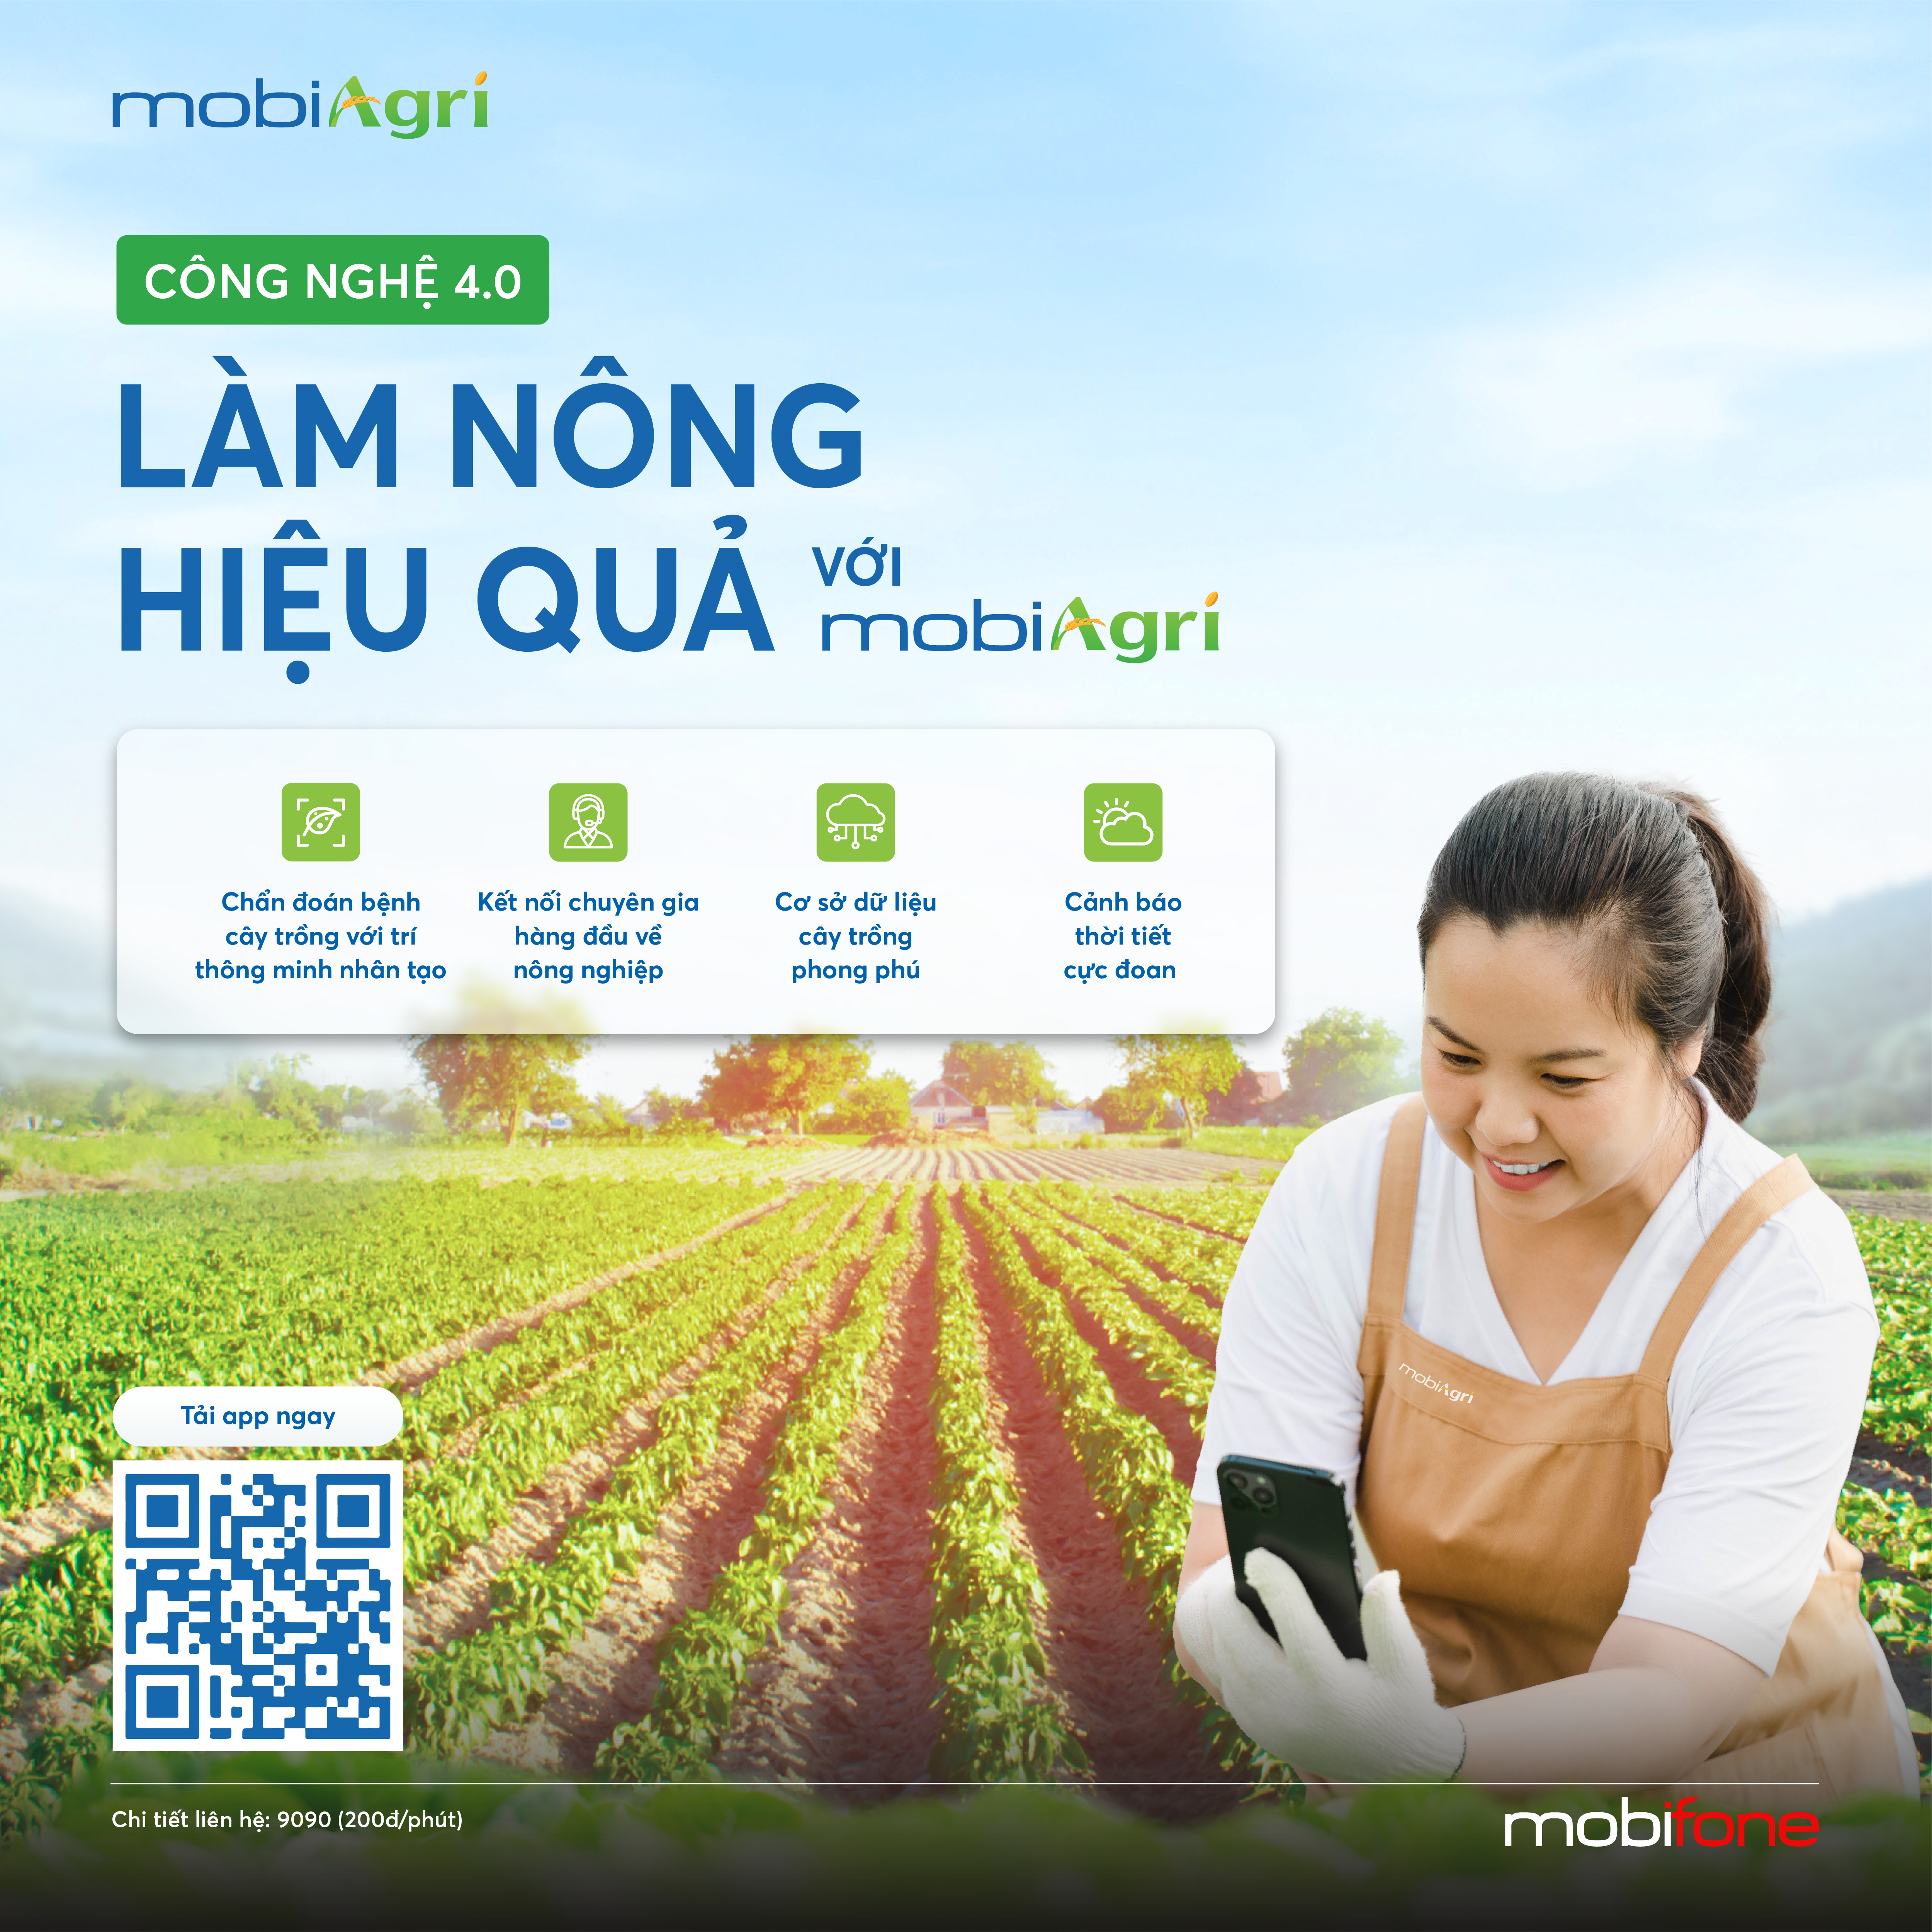
\includegraphics[width=0.9\textwidth]{img/MobiAgr.png}
    \caption{Giái pháp của MobiFone Smart Agriculture}
\end{figure}
\subsubsection*{MobiFone Smart Agriculture (mobiAgri)}
\begin{itemize}
\item Nền tảng nông nghiệp số đại chúng dựa trên 4G/5G.
\item AI chẩn đoán bệnh cây qua hình ảnh.
\item Kết nối chuyên gia và thiết bị IoT cơ bản.
\end{itemize}

\subsubsection*{CẠM BẪY CỦA GIẢI PHÁP DIY VÀ MÃ NGUỒN MỞ}
\subsubsection*{ThingsBoard và hệ lụy phân mảnh}
\begin{itemize}
\item Gánh nặng bảo trì và phụ thuộc đơn vị lắp đặt.
\item Độ bền cảm biến thấp, dễ sai số trong môi trường khắc nghiệt.
\item Thiếu mô hình nông học, khó chuyển dữ liệu thành quyết định canh tác.
\end{itemize}

\subsection{Khảo sát các mô hình, thuật toán, phương pháp}
\subsection{Bảng tổng hợp và phân tích khoảng trống}


\subsubsection*{3.3. Bảng tổng hợp và phân tích khoảng trống (Gap Analysis)}

Dựa trên khảo sát thực tế, bảng dưới đây so sánh các nhóm giải pháp theo các tiêu chí quan trọng đối với nhà quản lý phi kỹ thuật.

\medskip

\renewcommand{\arraystretch}{1.3}
\begin{tabularx}{\textwidth}{|p{3.2cm}|X|X|X|} % chktex 44
\hline % chktex 44
\textbf{Tiêu chí} &
\textbf{Giải pháp Quốc tế \newline (Netafim / Fujitsu)} &
\textbf{Giải pháp Trong nước \newline (Rynan / NextFarm / Mimosa)} &
\textbf{Giải pháp Viễn thông \newline (MobiFone)} \\
\hline % chktex 44

\textbf{Tính năng cốt lõi} &
Chuyên sâu về nông học: điều khiển dựa trên mô hình sinh lý cây trồng (Crop Models), tự động hóa gần như toàn bộ. &
Quản lý và giám sát: tập trung thu thập dữ liệu (Data Logging), điều khiển từ xa và quản lý quy trình (ERP). &
Thông tin và tư vấn: chẩn đoán bệnh bằng AI, thư viện kiến thức, kết nối chuyên gia. \\
\hline % chktex 44

\textbf{Trải nghiệm người dùng (UX)} &
Phức tạp: giao diện nhiều thông số kỹ thuật, phù hợp kỹ sư nông nghiệp (Agronomist). &
Thân thiện: tiếng Việt, trực quan hóa bằng màu sắc/icon, thiết kế Mobile-first. &
Rất đơn giản: dễ dùng như mạng xã hội, phù hợp người dùng phổ thông. \\
\hline % chktex 44

\textbf{Hiệu năng \& Độ bền} &
Chuẩn công nghiệp (Industrial Grade): độ bền $>$10 năm, hoạt động ổn định ngay cả khi mạng không ổn định. &
Khá (Standard): thiết bị đã được nhiệt đới hóa, phụ thuộc sóng 3G/4G. &
Phụ thuộc thiết bị: phần mềm ổn định nhưng phần cứng cảm biến thường ở mức cơ bản. \\
\hline % chktex 44

\textbf{Khả năng mở rộng (Scalability)} &
Khó và đắt: chi phí mở rộng theo module cao, hệ sinh thái đóng (Closed Ecosystem). &
Linh hoạt: dễ thêm bớt thiết bị, tích hợp được nhiều hãng phần cứng khác nhau. &
Hạn chế: thường bán theo gói cố định (Bundle), khó tùy biến sâu. \\
\hline % chktex 44

\textbf{Phù hợp với Việt Nam} &
Thấp: chi phí rất cao, yêu cầu hạ tầng nhà màng chuẩn. &
Cao: giá hợp lý, giải quyết đúng các “nỗi đau” địa phương (mặn, sâu rầy, nhân công). &
Trung bình: phù hợp giai đoạn khởi đầu nhưng thiếu chiều sâu quản trị. \\
\hline % chktex 44
\end{tabularx}

\medskip

\subsubsection*{Phân tích khoảng trống (Gap Analysis) và Cơ hội}

Từ bảng so sánh trên, nhóm nghiên cứu xác định ba khoảng trống lớn mà thị trường hiện tại chưa đáp ứng trọn vẹn cho nhóm khách hàng là nhà đầu tư và thương lái.

\subsubsection*{Khoảng trống về ``Bộ não Nông học'' (The Agronomic Intelligence Gap)}

\begin{itemize}
  \item \textbf{Vấn đề:} Các giải pháp trong nước làm tốt việc thu thập dữ liệu và thực thi (bật/tắt bơm), nhưng thiếu khả năng ra quyết định thay cho con người. Hệ thống chỉ báo trạng thái (ví dụ: đất khô) mà không tự tính được lượng tưới tối ưu theo giai đoạn sinh trưởng.
  \item \textbf{Nhu cầu chưa được đáp ứng:} Người quản lý phi kỹ thuật cần hệ thống không chỉ trả lời ``điều gì đang xảy ra'' mà còn đề xuất ``cần làm gì tiếp theo'' (Prescriptive Analytics) dựa trên quy trình chuẩn, với chi phí phù hợp thị trường Việt Nam.
\end{itemize}

\subsubsection*{Khoảng trống liên kết Tài chính -- Kỹ thuật (The Tech--Finance Disconnect)}

\begin{itemize}
  \item \textbf{Vấn đề:} Quản lý kỹ thuật (IoT) và quản lý tài chính đang bị tách rời. Người dùng biết số lần tưới nhưng không biết chi phí điện, nước, phân bón tương ứng ngay tại thời điểm vận hành.
  \item \textbf{Nhu cầu chưa được đáp ứng:} Một Dashboard hợp nhất (Unified Dashboard) hiển thị chi phí vận hành theo thời gian thực song song với chỉ số môi trường. Ví dụ: ``Độ ẩm thấp, đề xuất tưới. Chi phí dự kiến: 50.000 VNĐ''.
\end{itemize}

\subsubsection*{Khoảng trống về Dịch vụ vận hành (Operation-as-a-Service)}

\begin{itemize}
  \item \textbf{Vấn đề:} Khách hàng mua phần mềm và thiết bị nhưng vẫn gặp khó khăn trong vận hành hiệu quả. Mô hình tư vấn hiện tại chủ yếu dừng ở hỏi--đáp.
  \item \textbf{Cơ hội tiếp cận mới:} Mô hình ``Remote Agronomist'' -- kỹ sư nông nghiệp từ xa. Nhà cung cấp không chỉ bán phần mềm mà cung cấp gói giám sát vận hành, theo dõi Dashboard hàng ngày và đưa ra cảnh báo chuyên sâu, tương tự Fujitsu nhưng với chi phí phù hợp thị trường Việt Nam.
\end{itemize}
